\documentclass[
11pt, % The default document font size, options: 10pt, 11pt, 12pt
%codirector, % Uncomment to add a codirector to the title page
]{plan}




% El títulos de la memoria, se usa en la carátula y se puede usar el cualquier lugar del documento con el comando \ttitle
\titulo{Cámara de seguridad IoT con conectividad LoRaWAN}

% Nombre del posgrado, se usa en la carátula y se puede usar el cualquier lugar del documento con el comando \degreename
%\posgrado{Carrera de Especialización en Sistemas Embebidos}
%\posgrado{Carrera de Especialización en Internet de las Cosas}
%\posgrado{Carrera de Especialización en Intelegencia Artificial}
\posgrado{Maestría en Sistemas Embebidos}
%\posgrado{Maestría en Internet de las cosas}

% Tu nombre, se puede usar el cualquier lugar del documento con el comando \authorname
\autor{Esp. Ing. Mauricio Barroso Benavides}

% El nombre del director y co-director, se puede usar el cualquier lugar del documento con el comando \supname y \cosupname y \pertesupname y \pertecosupname
\director{Mg. Ing. Gonzalo Sanchez}
\pertenenciaDirector{FF.AA, FIUBA}
% FIXME:NO IMPLEMENTADO EL CODIRECTOR ni su pertenencia
\codirector{John Doe} % para que aparezca en la portada se debe descomentar la opción codirector en el documentclass
\pertenenciaCoDirector{FIUBA}

% Nombre del cliente, quien va a aprobar los resultados del proyecto, se puede usar con el comando \clientename y \empclientename
\cliente{Nombre del cliente}
\empresaCliente{Empresa del cliente}

% Nombre y pertenencia de los jurados, se pueden usar el cualquier lugar del documento con el comando \jurunoname, \jurdosname y \jurtresname y \perteunoname, \pertedosname y \pertetresname.
\juradoUno{Nombre y Apellido (1)}
\pertenenciaJurUno{pertenencia (1)}
\juradoDos{Nombre y Apellido (2)}
\pertenenciaJurDos{pertenencia (2)}
\juradoTres{Nombre y Apellido (3)}
\pertenenciaJurTres{pertenencia (3)}
\fechaINICIO{23 de junio de 2021}		%Fecha de inicio de la cursada de GdP \fechaInicioName
\fechaFINALPlan{11 de agosto de 2021} 	%Fecha de final de cursada de GdP
\fechaFINALTrabajo{15 de mayo de 2022}	%Fecha de defensa pública del trabajo final


\begin{document}

\maketitle
\thispagestyle{empty}
\pagebreak


\thispagestyle{empty}
{\setlength{\parskip}{0pt}
\tableofcontents{}
}
\pagebreak


\section*{Registros de cambios}
\label{sec:registro}


\begin{table}[ht]
\label{tab:registro}
\centering
\begin{tabularx}{\linewidth}{@{}|c|X|c|@{}}
\hline
\rowcolor[HTML]{C0C0C0}
Revisión & \multicolumn{1}{c|}{\cellcolor[HTML]{C0C0C0}Detalles de los cambios realizados} & Fecha      \\ \hline
0      & Creación del documento                                 &\fechaInicioName \\ \hline
1      & Se completa hasta el punto 5 inclusive                 & 13 de julio de 2021 \\
\hline
2      & Se completa hasta el punto 9 inclusive                 & 27 de julio de 2021 \\
\hline
3      & Se completa hasta el punto 11 inclusive                 & 4 de Agosto de 2021 \\
\hline
4      & Se completa hasta el punto 15 inclusive. Se deja pendiente el punto 14                 & 4 de Agosto de 2021 \\
\hline
5      & Se completa el punto 14                 & 10 de Agosto de 2021 \\
\hline
% 2      & Se completa hasta el punto 9 inclusive                 & 27 de julio de 2021 \\ \hline
%2      & Se completa hasta el punto 7 inclusive
%		  Se puede agregar algo más \newline
%		  En distintas líneas \newline
%		  Así                                                    & dd/mm/aaaa \\ \hline
%3      & Se completa hasta el punto 11 inclusive                & dd/mm/aaaa \\ \hline
%4      & Se completa el plan	                                 & dd/mm/aaaa \\ \hline
\end{tabularx}
\end{table}

\pagebreak



\section*{Acta de constitución del proyecto}
\label{sec:acta}

\begin{flushright}
Buenos Aires, \fechaInicioName
\end{flushright}

\vspace{2cm}

Por medio de la presente se acuerda con el \authorname\hspace{1px} que su Trabajo Final de la \degreename\hspace{1px} se titulará ``\ttitle'', consistirá esencialmente en la implementación de un prototipo de una cámara de seguridad para entornos IoT con conectividad LoRaWAN, y tendrá un presupuesto preliminar estimado de 600 hs de trabajo y US\$200, con fecha de inicio \fechaInicioName\hspace{1px} y fecha de presentación pública \fechaFinalName.

Se adjunta a esta acta la planificación inicial.

\vfill

% Esta parte se construye sola con la información que hayan cargado en el preámbulo del documento y no debe modificarla
\begin{table}[ht]
\centering
\begin{tabular}{ccc}
\begin{tabular}[c]{@{}c@{}}Ariel Lutenberg \\ Director posgrado FIUBA\end{tabular} & \hspace{2cm} & \begin{tabular}[c]{@{}c@{}}\supname \\ Director del Trabajo Final\end{tabular} \vspace{2.5cm} \\
%\multicolumn{3}{c}{\begin{tabular}[c]{@{}c@{}} \supname \\ Director del Trabajo Final\end{tabular}} \vspace{2.5cm} \\
%\begin{tabular}[c]{@{}c@{}}\jurunoname \\ Jurado del Trabajo Final\end{tabular}     &  & \begin{tabular}[c]{@{}c@{}}\jurdosname\\ Jurado del Trabajo Final\end{tabular}  \vspace{2.5cm}  \\
%\multicolumn{3}{c}{\begin{tabular}[c]{@{}c@{}} \jurtresname\\ Jurado del Trabajo Final\end{tabular}} \vspace{.5cm}                                                                    
\end{tabular}
\end{table}




\section{1. Descripción técnica-conceptual del proyecto a realizar}
\label{sec:descripcion}

La seguridad de espacios y bienes es un aspecto muy importante en la vida de las personas. Es así que en el mercado existen distintos tipos de soluciones basadas en dispositivos electrónicos, que permiten controlar y monitorear los espacios geográficos en donde se encuentran instalados. Estos dispositivos en conjunto forman sistemas de seguridad, que pueden detectar mediante distintos tipos de datos eventos no deseados.

Los dispositivos electrónicos de seguridad más utilizados son las cámaras. Estas permiten obtener imágenes en forma de videos o fotografías del sector en particular donde se encuentran. Los primeros sistemas de seguridad basados en cámaras necesitaban de un dispositivo para almacenar las imágenes que obtenían. Hoy en día las cámaras de seguridad poseen distintos tipos de conectividad hacia Internet, lo que les permite transmitir las imágenes que obtienen hacia servidores en la nube para que sean procesadas y almacenadas.

La transferencia de datos desde una cámara de seguridad hacia Internet requiere de un gran ancho de banda, por lo que es muy común que estos dispositivos posean conectividad Wi-Fi (inalámbrico) y/o Ethernet (cableado). La utilización de estas conexiones implica la existencia previa de, generalmente, una red de tipo LAN (Local Area Network) que consta principalmente de un router que se encarga de proporcionar direcciones IP (Internet Protocol) a todos los dispositivos de la red. Este escenario es muy común en entornos urbanos, donde, los proveedores de Internet proporcionan a sus usuarios conexiones estables y de gran ancho de banda, a través de redes de fibra óptica y/o cable coaxial.

Por otro lado, las zonas rurales no cuentan con la cobertura de los proveedores de Internet de las zonas urbanas, ya que a estos no les resulta rentable, y en muchos casos posible, instalar toda la infraestructura necesaria para proporcionar sus servicios. Para estos casos existen cámaras de seguridad con conectividad móvil (redes de telefonía) para transferir datos hacia Internet. Aunque esto supone un costo económico adicional que varía en función de la cantidad de datos transferidos, es una de las pocas soluciones viables que existen actualmente en el mercado. Es común también que este tipo de cámaras dispongan de una fuente de alimentación basada en baterías o paneles solares.

Entonces, el objetivo de este trabajo es diseñar e implementar una cámara de seguridad que pueda utilizarse en lugares donde no existen redes de banda ancha y tampoco una fuente de alimentación constante, y de esta manera lograr un dispositivo con la capacidad solucionar la problemática planteada previamente.

El desarrollo de este proyecto está basado principalmente en el área de sistemas embebidos, pero también incorpora elementos propios de IoT (Internet of Things) y ML (Machine Learning) para lograr prestaciones adecuadas al contexto actual. El Internet de las cosas o IoT, por sus siglas en inglés, se refiere a la conexión de dispositivos y objetos a Internet con el objetivo de monitorearlos e interactuar con ellos de manera remota. IoT plantea algunas problemáticas como la seguridad de la información, la alimentación de dispositivos que no disponen de una fuente de energía eléctrica constante y la administración del ancho de banda disponible. El aprendizaje automático o ML, por sus siglas en inglés, permite a los sistemas computacionales realizar predicciones y tomar decisiones en función de los datos de entrada. En los últimos años la optimización que han tenido los algoritmos de ML permiten que estos puedan ser ejecutados en sistemas embebidos, lo que da como resultado una amplia gama de nuevas aplicaciones y otra perspectiva para resolver problemas antes planteados.

Dentro de un entorno IoT elegir el tipo de red para la interconexión de nodos finales con Internet es un aspecto muy importante. Es así que, en aplicaciones donde el consumo energético y el aprovechamiento de ancho de banda son importantes, LoRaWAN es el tipo de red óptimo para estos casos. Esta red permite la conexión de nodos finales hacia gateways conectados a Internet hasta una distancia teórica de 20 Km y con un ancho de banda de hasta 500 KHz (US915). La topología de red a utilizar en este proyecto sería la que se observa en la figura \ref{fig:topology}.

\begin{figure}[htpb]
\centering
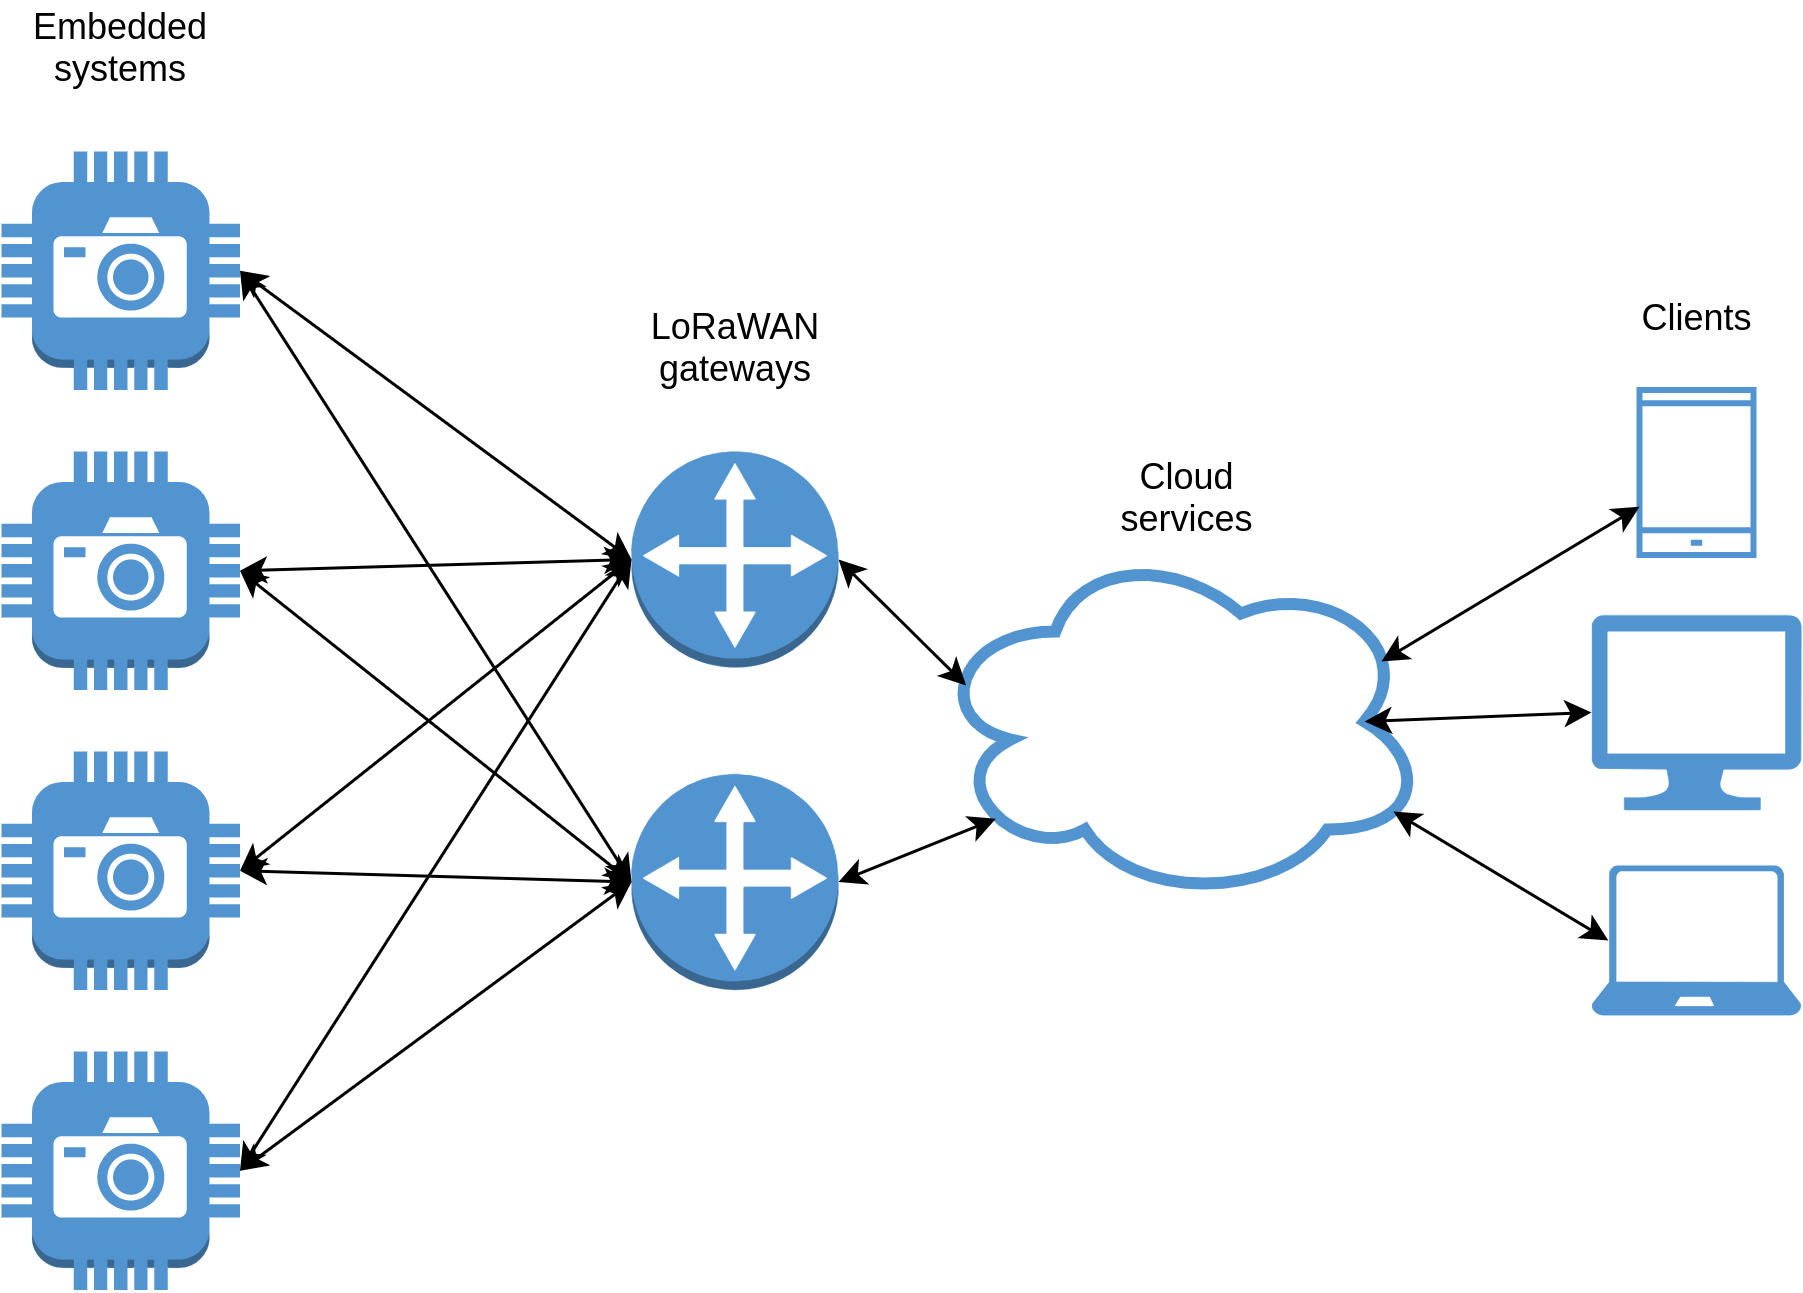
\includegraphics[width=0.8\textwidth]{./fig/topology.png}
\caption{Diagrama en bloques del sistema}
\label{fig:topology}
\end{figure}

\vspace{25px}

Según todas las características antes descritas, el sistema embebido implicado en este trabajo deberá tener el diagrama de bloques que se expone en la figura \ref{fig:blocks}.

\begin{figure}[htpb]
\centering
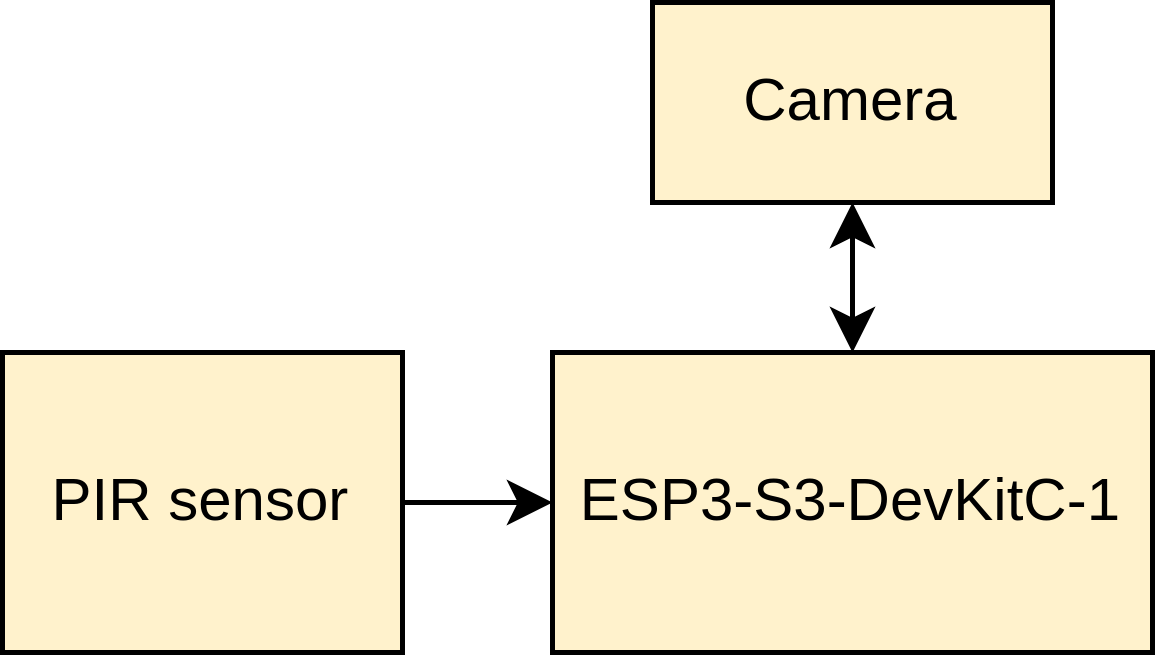
\includegraphics[width=0.5\textwidth]{./fig/blocks.png}
\caption{Diagrama en bloques del sistema}
\label{fig:blocks}
\end{figure}

\vspace{25px}

El sistema embebido tiene como componente más importante un microcontrolador que se encarga principalmente de ejecutar un modelo de machine learning para la detección de personas, sus entradas son los valores leídos por la cámara y el sensor de movimiento PIR (Passive InfraRed). Otra función del microcontrolador es la ejecución del stack LoRaWAN, para que en conjunto con el transceptor LoRa, el sistema pueda interactuar correctamente dentro de una red de este tipo. Finalmente, se cuenta con una tarjeta SD (Secure Digital) para almacenar las imágenes capturadas por la cámara.

\section{2. Identificación y análisis de los interesados}
\label{sec:interesados}

\begin{table}[ht]
%\caption{Identificación de los interesados}
%\label{tab:interesados}
\begin{tabularx}{\linewidth}{@{}|l|X|X|l|@{}}
\hline
\rowcolor[HTML]{C0C0C0}
Rol           & Nombre y Apellido & Organización 			& Puesto 	\\ \hline
Responsable   & \authorname		& -        				& Alumno 	\\ \hline
Orientador    & \supname			& - 						& Director Trabajo final \\ \hline
Usuario final & -                 & -             			& -       	\\ \hline
\end{tabularx}
\end{table}

\begin{itemize}
	\item Orientador: Tiene la capacidad de ayudar al alumno a resolver los problemas técnicos y conceptuales que se presenten a lo largo del proyecto. Es exigente con los tiempos y la calidad del desarrollo del proyecto.
	\item Usuario final: No posee conocimientos sobre sistemas embebidos y las tecnologías utilizadas en el proyecto, y espera dispositivos de bajo costo económico.
\end{itemize}



\section{3. Propósito del proyecto}
\label{sec:proposito}

El propósito de este proyecto es diseñar e implementar un sistema embebido que funcione como cámara de seguridad en un entorno IoT con ayuda de algoritmos de ML.

Un propósito personal del autor es obtener conocimientos y experiencia sobre implementación de algoritmos de ML en sistemas embebidos.

\section{4. Alcance del proyecto}
\label{sec:alcance}

Este proyecto incluye:
\begin{itemize}
	\item Diseño e implementación del firmware del sistema embebido.
	\item Diseño e implementación del algoritmo de ML para reconocimiento de personas.
	\item Implementación del sistema embebido desarrollado dentro de una arquitectura IoT existente.
	\item Diseño del PCB para el prototipo funcional del sistema embebido.
	\item Creación de documentación sobre datos técnicos y características del sistema embebido.
\end{itemize}

Este proyecto no incluye:
\begin{itemize}
	\item Implementación del PCB para el prototipo funcional del sistema embebido.
	\item Desarrollo de una aplicación para el usuario final.
\end{itemize}

\section{5. Supuestos del proyecto}
\label{sec:supuestos}

\begin{itemize}
	\item Se contará con el presupuesto necesario para obtener los componentes del proyecto.
	\item Se dedicarán al menos 2 horas diarias para la realización del proyecto.
	\item Se dispondrá de una arquitectura IoT para redes LoRaWAN para la realización de pruebas y puesta en marcha del proyecto.
\end{itemize}

\section{6. Requerimientos}
\label{sec:requerimientos}

El presente proyecto tiene dos tipos de requerimientos, funcionales y no funcionales. A continuación se citan los antes referidos.

\begin{enumerate}
	\item Requerimientos funcionales
		\begin{enumerate}
			\item El sistema debe conectarse a una red LoRaWAN en la banda de frecuencia AU915 como dispositivo de clase A.
			\item El sistema debe ser alimentado mediante dos baterías de tipo AA.
			\item El sistema debe poseer mecanismos de seguridad implementados tanto en hardware como en software para evitar su manipulación incorrecta.
			\item El sistema debe almacenar fotografías y videos obtenidos mediante su cámara cámara en una memoria no volátil.
			\item El sistema debe recibir su configuración inicial mediante interruptores físicos conectados al mismo.
			\item El sistema debe recibir sus parámetros de funcionamiento mediante la red LoRaWAN a la que está conectada.
			\item El sistema debe funcionar solamente si se detecta movimiento en el sector donde se encuentra instalada.
			\item El sistema debe ser compatible con la especificación LoRaWAN 1.0.2.
			\item El sistema debe, con ayuda de su cámara, detectar la presencia de personas a través de un algoritmo de ML.
		\end{enumerate}
	\item Requerimientos no funcionales
		\begin{enumerate}
			\item El sistema deberá tener un costo de desarrollo igual o menor a 200U\$S.
			\item El sistema deberá tener documentación adecuada sobre su uso y desarrollo.
		\end{enumerate}
\end{enumerate}

\section{7. Historias de usuarios (\textit{Product backlog})}
\label{sec:backlog}

El criterio para determinar los \textit{storyboards} es el siguiente.

\begin{itemize}
	\item Complejidad
	\begin{itemize}
		\item Alto: 5
		\item Medio: 3
		\item Bajo: 1
	\end{itemize}
	\item Tiempo
	\begin{itemize}
		\item Alto: 5
		\item Medio: 3
		\item Bajo: 1
	\end{itemize}
	\item Recursos
	\begin{itemize}
		\item Alto: 5
		\item Medio: 3
		\item Bajo: 1
	\end{itemize}
\end{itemize}

\begin{enumerate}
	\item Como usuario quiero que la duración de las baterías sea al menos de 1 año para que no suponga un costo económico adicional muy alto.
	\begin{itemize}
		\item Complejidad: 3
		\item Tiempo: 4
		\item Recursos: 1
	\end{itemize}
	\item Como usuario quiero que la configuración del sistema se haga en pocos pasos para evitar complicaciones en su puesta en marcha.
	\begin{itemize}
		\item Complejidad: 4
		\item Tiempo: 4
		\item Recursos: 1
	\end{itemize}
	\item Como desarrollador del firmware quiero que el sistema esté basado en un RTOS(Real Time Operating System) para poder escalar la aplicación de manera más sencilla.
	\begin{itemize}
		\item Complejidad: 3
		\item Tiempo: 4
		\item Recursos: 1
	\end{itemize}
\end{enumerate}

\section{8. Entregables principales del proyecto}
\label{sec:entregables}

Los entregables del proyecto son:

\begin{itemize}
	\item Repositorio en Github con el código fuente.
	\item Prototipo de pruebas del sistema embebido.
	\item Informe final.
\end{itemize}

\section{9. Desglose del trabajo en tareas}
\label{sec:wbs}

\begin{enumerate}
\item Análisis y planificación preliminar (122 hs)
	\begin{enumerate}
		\item Planificar el proyecto. (38 hs)
		\item Investigar sobre sistemas similares. (24 hs)
		\item Definir los componentes a utilizar. (6 hs)
		\item Recopilar y estudiar documentos (datasheets y application notes) de los componentes a utilizar. (30 hs)
		\item Investigar las normativas locales sobre redes que utilizan las bandas ISM(Industrial, Scientific and Medical). (12 hs)
		\item Planificar y diagramar la arquitectura a utilizar en el sistema (10 hs)
		\item Crear un repositorio en la nube para almacenar el código a desarrollar (2 hs)
	\end{enumerate}
	
\item Prototipo de pruebas (40 hs)
	\begin{enumerate}
		\item Obtener los componentes del sistema. (12 hs)
		\item Probar la funcionalidad de todos los componentes del sistema por separado. (26 hs)
		\item Montar el prototipo de pruebas y asegurar conexiones. (2 hs)
	\end{enumerate}
	
\item LoRaWAN (66 hs)
	\begin{enumerate}
		\item Desarrollar código para el stack LoRaWAN. (22 hs)
		\item Desarrollar código para configurar el sistema como dispositivo LoRaWAN de clase A. (18 hs)
		\item Desarrollar código para enviar y recibir paquetes de datos a través de una red LoRaWAN en la banda AU915. (16 hs)
		\item Probar el código desarrollado en el prototipo de pruebas. (10 hs)
	\end{enumerate}
	
\item ML (148 hs)
	\begin{enumerate}
		\item Realizar un curso sobre TinyML. (40 hs)
		\item Desarrollar el modelo de ML a utilizar. (30 hs)
		\item Desarrollar código para integrar el modelo de ML en el sistema. (32 hs)
		\item Desarrollar una biblioteca de código para controlar la cámara del sistema. (24 hs)
		\item Desarrollar código para integrar la cámara del sistema con el modelo de ML. (12 hs)
		\item Probar el código desarrollado en el prototipo de pruebas. (10 hs)
	\end{enumerate}

\item IoT (82 hs)
	\begin{enumerate}
		\item Configurar el entorno IoT para integrar al sistema. (14 hs)
		\item Definir el formato de los paquetes a recibir y transmitir. (2 hs)
		\item Desarrollar código para integrar el código de LoRaWAN y ML. (48 hs).
		\item Probar el código desarrollado en el prototipo de pruebas. (10 hs)
		\item Implementar el prototipo de pruebas dentro del entorno IoT. (8 hs)
	\end{enumerate}
	
\item V\&V (48 hs)
	\begin{enumerate}
		\item Medir y comprobar los parámetros eléctricos del sistema con instrumentos de laboratorio. (8 hs)
		\item Probar el sistema en un entorno de trabajo controlado. (36 hs)
		\item Analizar las experiencias de uso reportadas por los usuarios. (4 hs)
	\end{enumerate}
	
\item Cierre (106 hs)
	\begin{enumerate}
		\item Elaborar la memoria técnica del trabajo final. (80 hs)
		\item Elaborar la presentación del trabajo final. (26 hs)
	\end{enumerate}
\end{enumerate}

Cantidad total de horas: (612 hs)

\section{10. Diagrama de Activity On Node}
\label{sec:AoN}

El diagrama de actividades se puede observar en la figura \ref{fig:AoN}.

\begin{figure}[htpb]
\centering
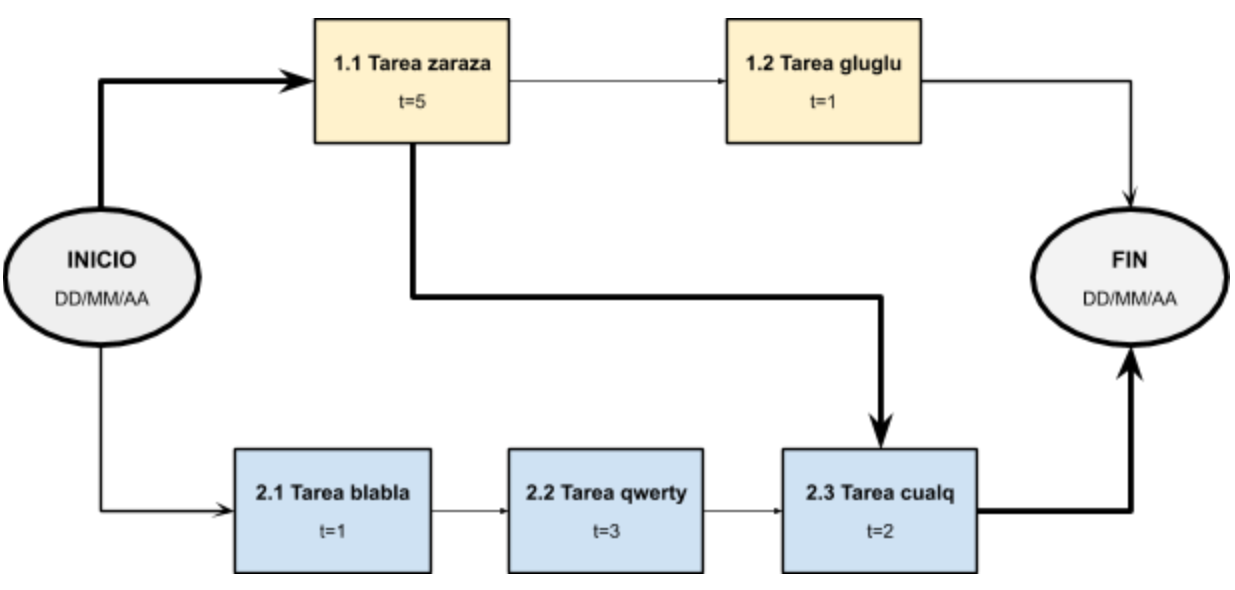
\includegraphics[width=.6\textwidth]{./fig/AoN.png}
\caption{Diagrama en \textit{Activity on Node}}
\label{fig:AoN}
\end{figure}

\section{11. Diagrama de Gantt}
\label{sec:gantt}

En la figura \ref{sec:gantt} se puede observar el diagrama de Gantt de este proyecto.

\begin{landscape}
\begin{figure}[htpb]
\centering
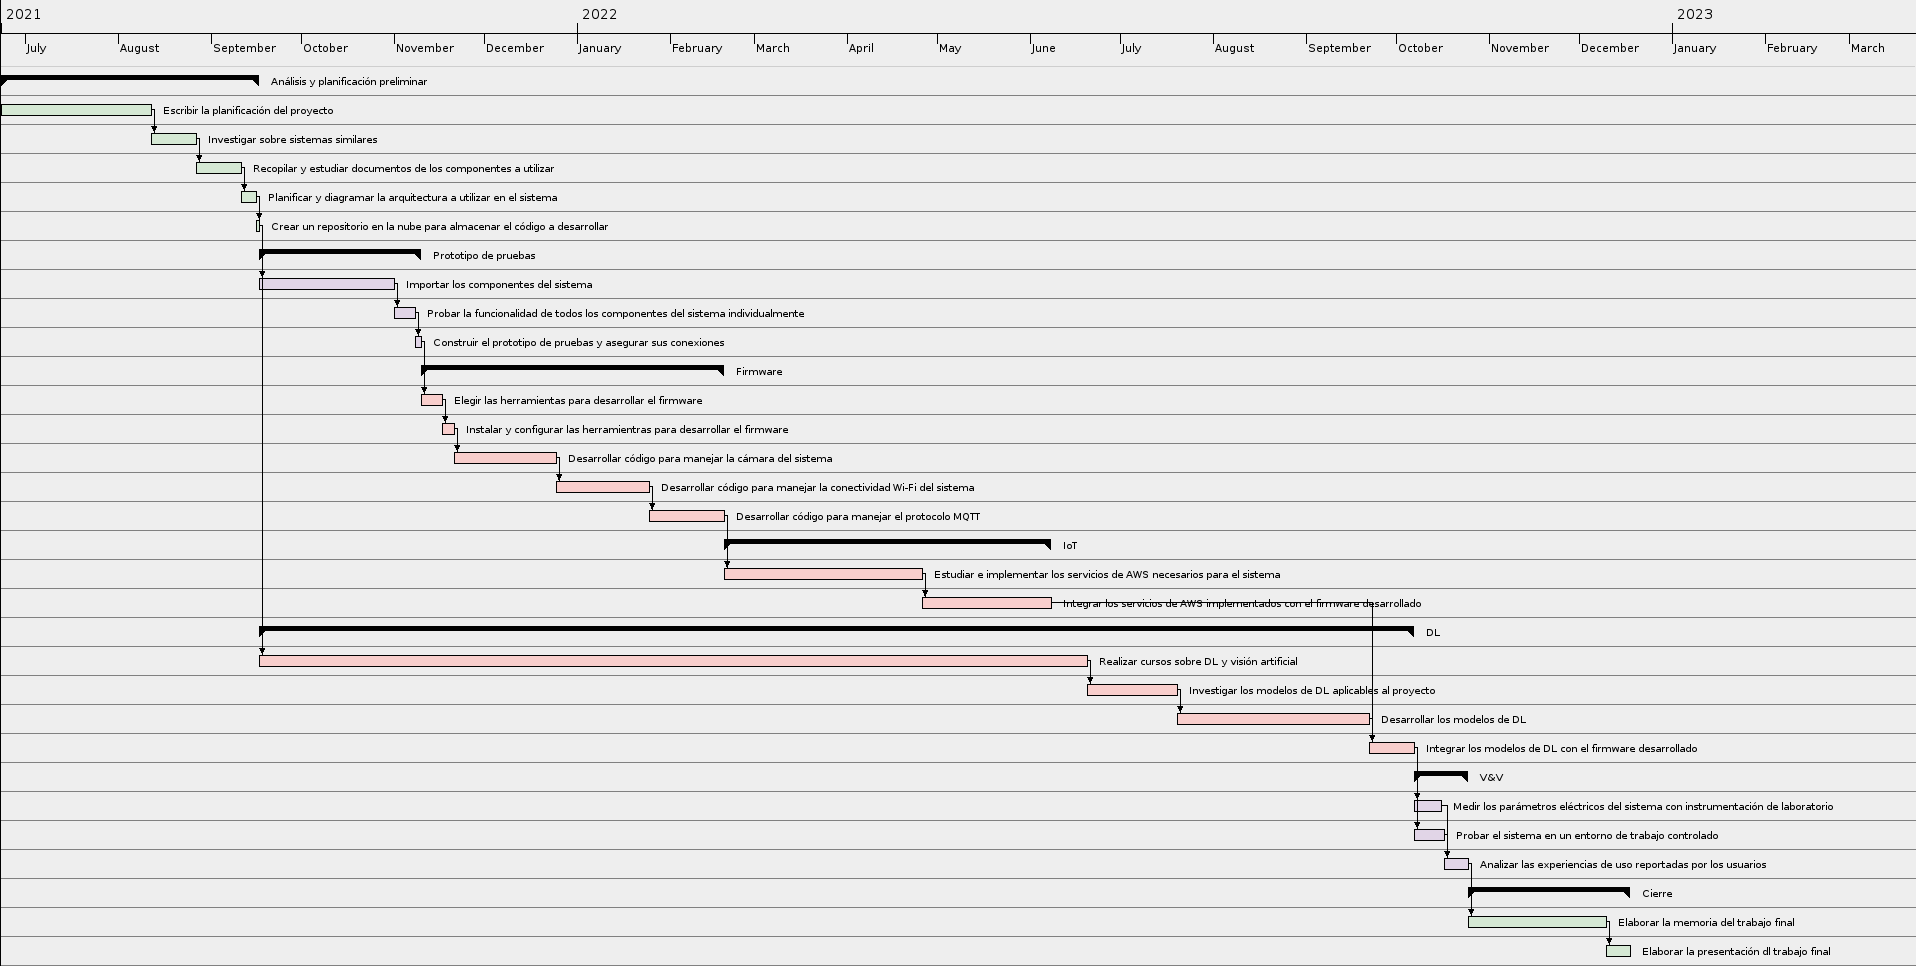
\includegraphics[height=.95\textheight]{./fig/gantt.png}
\caption{Diagrama de Gantt}
\label{fig:diagGantt}
\end{figure}

\end{landscape}



\section{12. Presupuesto detallado del proyecto}
\label{sec:presupuesto}

El presupuesto que se presenta en esta sección es un aproximado, ya que valores de los componentes que son parte del sistema embebido aún no fueron definidos. Por tanto, se consideran los costos más altos del mercado de componentes que cumplan las funciones requeridas. De esta manera se tiene un presupuesto suficiente para cumplir con el proyecto.

\begin{table}[htpb]
\centering
\begin{tabularx}{\linewidth}{@{}|X|c|r|r|@{}}
\hline
\rowcolor[HTML]{C0C0C0}
\multicolumn{4}{|c|}{\cellcolor[HTML]{C0C0C0}COSTOS DIRECTOS} \\ \hline
\rowcolor[HTML]{C0C0C0}
Descripción &
 \multicolumn{1}{c|}{\cellcolor[HTML]{C0C0C0}Cantidad} &
 \multicolumn{1}{c|}{\cellcolor[HTML]{C0C0C0}Valor unitario} &
 \multicolumn{1}{c|}{\cellcolor[HTML]{C0C0C0}Valor total} \\ \hline
\multicolumn{1}{|l|}{Placa de desarrollo de ST (ARM Cortex M4)} &
\multicolumn{1}{|c|}{1} &
\multicolumn{1}{|c|}{47} &
\multicolumn{1}{|c|}{47}
  \\ \hline
\multicolumn{1}{|l|}{Módulo con cámara de 5 megapixeles} &
\multicolumn{1}{|c|}{1} &
\multicolumn{1}{|c|}{45} &
\multicolumn{1}{|c|}{45}
  \\ \hline
\multicolumn{1}{|l|}{Módulo transceptor LoRaWAN US915} &
\multicolumn{1}{|c|}{1} &
\multicolumn{1}{|c|}{25} &
\multicolumn{1}{|c|}{25}
  \\ \hline
\multicolumn{1}{|l|}{Módulo para tarjeta SD} &
\multicolumn{1}{|c|}{1} &
\multicolumn{1}{|c|}{3} &
\multicolumn{1}{|c|}{3}
  \\ \hline
\multicolumn{1}{|l|}{Módulo sensor PIR} &
\multicolumn{1}{|c|}{1} &
\multicolumn{1}{|c|}{2} &
\multicolumn{1}{|c|}{2}
  \\ \hline
\multicolumn{1}{|l|}{Módulo para tarjeta SD} &
\multicolumn{1}{|c|}{1} &
\multicolumn{1}{|c|}{3} &
\multicolumn{1}{|c|}{3}
  \\ \hline
\multicolumn{1}{|l|}{Otros (cables, conectores, etc)} &
\multicolumn{1}{|c|}{1} &
\multicolumn{1}{|c|}{10} &
\multicolumn{1}{|c|}{10}
  \\ \hline
\multicolumn{3}{|c|}{SUBTOTAL} &
 \multicolumn{1}{c|}{135} \\ \hline
\rowcolor[HTML]{C0C0C0}
\multicolumn{4}{|c|}{\cellcolor[HTML]{C0C0C0}COSTOS INDIRECTOS} \\ \hline
\rowcolor[HTML]{C0C0C0}
Descripción &
 \multicolumn{1}{c|}{\cellcolor[HTML]{C0C0C0}Cantidad} &
 \multicolumn{1}{c|}{\cellcolor[HTML]{C0C0C0}Valor unitario} &
 \multicolumn{1}{c|}{\cellcolor[HTML]{C0C0C0}Valor total} \\ \hline
\multicolumn{1}{|l|}{50\% del costo directo} &
\multicolumn{1}{|c|}{1} &
\multicolumn{1}{|c|}{67,5} &
\multicolumn{1}{|c|}{67,5}
  \\ \hline
\multicolumn{3}{|c|}{SUBTOTAL} &
 \multicolumn{1}{c|}{67,5} \\ \hline
\rowcolor[HTML]{C0C0C0}
\multicolumn{3}{|c|}{TOTAL} &
\multicolumn{1}{|c|}{202,5}
  \\ \hline
\end{tabularx}%
\end{table}

Los valores expuestos en la tabla anterior están expresados en dólares americanos (U\$S). Esto se debe a que la mayor parte de los componentes serán importados directamente de proveedores en Estados Unidos.

\section{13. Gestión de riesgos}
\label{sec:riesgos}

a) Identificación de los riesgos y estimación de sus consecuencias:
Riesgo 1: Imposibilidad de obtener los componentes necesarios.
\begin{itemize}
	\item Severidad (S): 7. El sistema podría no funcionar de acuerdo a lo planificado.
	\item Probabilidad de ocurrencia (O): 3. Si no se encuentran los componentes en el mercado local, estos pueden ser importados
\end{itemize}  

Riesgo 2: El tamaño del modelo de ML puede sobrepasar la cantidad de memoria del microcontrolador.
\begin{itemize}
	\item Severidad (S): 9. Si el modelo de ML no puede ser almacenado en la memoria del microcontrolador, el sistema no podría realizar las funciones para las que fue planificado.
	\item Ocurrencia (O): 7. El tamaño del modelo de ML alcanzará un tamaño no adecuado en función de su complejidad.
\end{itemize}

Riesgo 3: Imposibilidad de contar con instrumentación de laboratorio.
\begin{itemize}
	\item Severidad (S): 3. Las mediciones de alta precisión son para contar con datos técnicos exactos, que ayudarán a desarrollar una versión comercial del sistema posteriormente.
	\item Ocurrencia (O): 2. En el lugar de residencia se cuenta con un laboratorio de electrónica que funciona regularmente y está abierto al público previa aceptación de los encargados.
\end{itemize}

Riesgo 4: Imposibilidad de contar con los recursos económicos necesarios.
\begin{itemize}
	\item Severidad (S): 10. No contar con el dinero necesario para comprar los componentes del sistema impediría la realización del proyecto.
	\item Ocurrencia (O): 2. El presupuesto requerido para el proyecto es relativamente bajo y son recursos que ya se tienen reservados.
\end{itemize}

Riesgo 5: Falta de tiempo para concluir el proyecto.
\begin{itemize}
	\item Severidad (S): 5. Si el proyecto no se concluye en las fechas planificadas, existe la posibilidad de que se retrase indefinidamente si se presentan otros proyectos más de mayor prioridad.
	\item Ocurrencia (O): 6. Por cuestiones tanto laborales como familiares el proyecto podría retrasarse de manera imprevista.
\end{itemize}

b) Tabla de gestión de riesgos:      (El RPN se calcula como RPN=SxO)

\begin{table}[htpb]
\centering
\begin{tabularx}{\linewidth}{@{}|X|c|c|c|c|c|c|@{}}
\hline
\rowcolor[HTML]{C0C0C0}
Riesgo & S & O & RPN & S* & O* & RPN* \\ \hline
Imposibilidad de obtener los componentes necesarios & 7 & 3 & 21 & - & - & -\\ \hline
El tamaño del modelo de ML puede sobrepasar la cantidad de memoria del microcontrolador & 9 & 7 & 63 & 9 & 2 & 18\\ \hline
Imposibilidad de contar con instrumentación de laboratorio & 3 & 2 & 6 & - & - & -\\ \hline
Imposibilidad de contar con los recursos económicos necesarios & 10 & 2 & 20 & - & - & -\\ \hline
Falta de tiempo para concluir el proyecto & 5 & 6 & 30 & 5 & 4 & 20\\ \hline
\end{tabularx}%
\end{table}

Criterio adoptado:
Se tomarán medidas de mitigación en los riesgos cuyos números de RPN sean mayores a 25.

c) Plan de mitigación de los riesgos que originalmente excedían el RPN máximo establecido:
Riesgo 2: Se realizará un curso de ML en microcontroladores durante el periodo de vacaciones.
\begin{itemize}
	\item Severidad (S): 9. Este riesgo sigue siendo muy severo por más conocimientos de ML que se posean.
	\item Ocurrencia (O): 2. Con los conocimientos adecuados sobre ML en microcontroladores se pueden optimizar estos algoritmos, de tal forma que pueden adaptarse a la cantidad de memoria del microcontrolador a utilizar. \\ \\
\end{itemize}
Riesgo 5: Durante el tiempo planificado del proyecto se trabajarán los fines de semana y feriados 4 horas diarias.
\begin{itemize}
	\item Severidad (S): 5. La severidad no se ve afectada por la medida de mitigación.
	\item Ocurrencia (O): 4. Las horas extras que se destinarán al proyecto podrían asegurar su conclusión en el tiempo planificado. Su ocurrencia baja muy poco porque no se descarta la posibilidad de que surjan imprevistos que retrasen el proyecto.
\end{itemize}

\section{14. Gestión de la calidad}
\label{sec:calidad}



\begin{enumerate}
	\item Requerimientos funcionales
		\begin{itemize}
			\item Req \#1.1: el sistema debe conectarse a una red LoRaWAN en la banda de frecuencia AU915 como dispositivo de clase A.

			\begin{itemize}
				\item Verificación: conectar el sistema a un servidor LNS (LoRaWAN Network Server) mediante un gateway LoRaWAN en la banda AU915 para comprobar a través de la UART que los paquetes son enviados correctamente y que los datos solo son recibidos mientras las ventanas de tiempo de recepción de los dispositivos clase A están disponibles.
				\item Validación: conectar el sistema a una arquitectura IoT existente a través de un gateway LoRaWAN comercial en la banda AU915 para enviar y recibir datos.
			\end{itemize}

		\end{itemize}
		
		\begin{itemize}
			\item Req \#1.2: el sistema debe ser alimentado mediante dos baterías de tipo AA.

			\begin{itemize}
				\item Verificación: con ayuda de un multímetro de precisión medir que los parámetros eléctricos requeridos por los componentes del sistema sean los requeridos por sus datasheets.
				\item Validación: visualizar el buen funcionamiento del sistema a través de los LEDs de estado disponibles.
			\end{itemize}

		\end{itemize}
		
		\begin{itemize}
			\item Req \#1.3: el sistema debe poseer mecanismos de seguridad implementados tanto en hardware como en software para evitar su manipulación incorrecta.

			\begin{itemize}
				\item Verificación: mediante herramientas proporcionadas por el fabricante de la tarjeta de desarrollo, comprobar que los sectores de memoria dedicados a la seguridad funcionen correctamente.
				\item Validación: intentar leer la memoria de programa del sistema y comprobar que no es posible.
			\end{itemize}

		\end{itemize}
		
		\begin{itemize}
			\item Req \#1.4: el sistema debe almacenar fotografías y videos obtenidos mediante su cámara cámara en una memoria no volátil.

			\begin{itemize}
				\item Verificación: verificar con ayuda de herramientas de depuración que los procesos de lectura y escritura entre el sistema y la tarjeta SD se realizan con éxito.
				\item Validación: probar el sistema y posteriormente extraer la tarjeta SD para visualizar las imágenes obtenidas a través de un adaptador USB y una PC.
			\end{itemize}

		\end{itemize}
		
		\begin{itemize}
			\item Req \#1.5: el sistema debe recibir su configuración inicial mediante interruptores físicos conectados al mismo.

			\begin{itemize}
				\item Verificación: mediante herramientas de depuración comprobar que los sectores de memoria donde se almacena la configuración de sistema conrrespondan con las posiciones de los interruptores físicos.
				\item Validación: configurar el sistema en sus diferentes modos a través de los interruptores físicos.
			\end{itemize}

		\end{itemize}
		
		\begin{itemize}
			\item Req \#1.6: el sistema debe recibir sus parámetros de funcionamiento mediante la red LoRaWAN a la que está conectada.

			\begin{itemize}
				\item Verificación: mediante herramientas de depuración comprobar que los sectores de memoria donde se almacena la configuración de sistema corresponda con los datos que se reciben por el servidor LNS.
				\item Validación: configurar el sistema en sus diferentes modos a través de una plataforma web.
			\end{itemize}

		\end{itemize}
		
		\begin{itemize}
			\item Req \#1.7: el sistema debe funcionar solamente si se detecta movimiento en el sector donde se encuentra instalada.

			\begin{itemize}
				\item Verificación: con ayuda del puerto UART imprimir el estado del sistema y la detección de movimiento a través del sensor PIR del sistema.
				\item Validación: determinar si los LEDs de estado del sistema son activados por el movimiento de algún cuerpo que se encuentre en el área del sistema.
			\end{itemize}

		\end{itemize}
		
		\begin{itemize}
			\item Req \#1.8: el sistema debe ser compatible con la especificación LoRaWAN 1.0.2.

			\begin{itemize}
				\item Verificación: utilizar herramientas para probar la compatibilidad de dispositivos LoRaWAN provistas por LoRa Alliance.
				\item Validación: conectar el sistema a una red LoRaWAN existente que cumpla con la especificación LoRaWAN 1.0.2.
			\end{itemize}

		\end{itemize}
		
		\begin{itemize}
			\item Req \#1.9: el sistema debe, con ayuda de su cámara, detectar la presencia de personas a través de un algoritmo de ML.

			\begin{itemize}
				\item Verificación: probar el algoritmo de ML mediante simuladores y con ayuda del puerto UART comprobar que se detecta correctamente la presencia de personas.
				\item Validación: probar el sistema en un entorno real de trabajo y con ayuda de una plataforma web comprobar la detección de personas.
			\end{itemize}

		\end{itemize}
		
	\item Requisitos no funcionales
	
		\begin{itemize}
			\item Req \#2.1: el sistema deberá tener un costo de desarrollo igual o menor a 200U\$S.

			\begin{itemize}
				\item Verificación: realizar la suma de los costos de cada componente para determinar que no se superó el presupuesto previamente propuesto.
				\item Validación: realizar un detalle de los costos del sistema.
			\end{itemize}

		\end{itemize}
		
		\begin{itemize}
			\item Req \#2.2: el sistema deberá tener documentación adecuada sobre su uso y desarrollo.

			\begin{itemize}
				\item Verificación: comprobar que los datos técnicos de los documentos sean consistentes con los datasheets y application notes de los componentes utilizados.
				\item Validación: presentar los documentos del proyecto a los directos interesados (director del trabajo, docentes y jurados).
			\end{itemize}

		\end{itemize}

\end{enumerate}

\section{15. Procesos de cierre}   
\label{sec:cierre}

Establecer las pautas de trabajo para realizar una reunión final de evaluación del proyecto, tal que contemple las siguientes actividades:

\begin{itemize}
	\item Pautas de trabajo que se seguirán para analizar si se respetó el Plan de Proyecto original:
		\begin{itemize}
			\item Responsable: Mauricio Barroso Benavides.
			\item Actividad: evaluar si se cumplieron los requerimientos del proyecto y las fechas planificadas.
		\end{itemize}
	\item Identificación de las técnicas y procedimientos útiles e inútiles que se emplearon, y los problemas que surgieron y cómo se solucionaron:
		\begin{itemize}
			\item Responsable: Mauricio Barroso Benavides.
			\item Actividad: evaluar las herramientas y metodologías para el desarollo de software y hardware del proyecto, para establecer las técnicas y procedimientos que se seguirán en proyectos futuros.
		\end{itemize}
	\item Indicar quién organizará el acto de agradecimiento a todos los interesados, y en especial al equipo de trabajo y colaboradores:
		\begin{itemize}
			\item Responsable: Mauricio Barroso Benavides.
			\item Actividad: agradecer públicamente a los profesores y responsables de la maestría, y a todos los involucrados en la realización del proyecto durante la defensa formal del mismo.
		\end{itemize}
\end{itemize}

\end{document}


